\section{Regresión lineal}

En una regresión lineal simple, hablamos acerca de la relación lineal entre una variable independiente y una variable dependiente. En este apéndice

\begin{description}
	\item[Regresión múltiple] Las relaciones lineales entre dos o más variables independientes y una variable dependiente.
	\item[Regresión polinomial] Modela la relación entre una variable independiente y una variable dependiente usando una función polinomial de grado $n$-ésimo.
	\item[Regresión polinomial múltiple] Modela la relación entre dos o más variables independientes y una variable dependiente usando una función polinomial de grado $n$-ésimo.
\end{description}

En la estadística, la \emph{regresión lineal} es uno de los más simples algoritmos que puede emplear a conjunto de datos para relacionar entre las características y sus etiquetas. En el
% TODO: Mencionar donde se usó la regresión lineal
donde se pudo explicar la relación entre la característica y una etiqueta usando una recta. En la siguiente sección, aprendará acerca de una variante de una regresión lineal simple, llamada \emph{regresión lineal múltiple}, para predecir los precios de las casas basadas en múltiples características.

\subsection{Usando el conjunto de datos de Boston}
Para este ejemplo, aprenderá a usar el conjunto de datos de Boston, el cual contiene datos acerca del alquiler y datos del precio en el área de Boston. Este conjunto de datos fue tomado de la StatLib

\begin{pygments}{pycon}
>>> import matplotlib.pyplot as plt
>>> import pandas as pd
>>> import numpy as np
>>> from sklearn.datasets import load_boston
>>> dataset = load_boston()
>>> print(dataset.data)
[[6.3200e-03 1.8000e+01 2.3100e+00 ... 1.5300e+01 3.9690e+02 4.9800e+00]
[2.7310e-02 0.0000e+00 7.0700e+00 ... 1.7800e+01 3.9690e+02 9.1400e+00]
[2.7290e-02 0.0000e+00 7.0700e+00 ... 1.7800e+01 3.9283e+02 4.0300e+00]
...
[6.0760e-02 0.0000e+00 1.1930e+01 ... 2.1000e+01 3.9690e+02 5.6400e+00]
[1.0959e-01 0.0000e+00 1.1930e+01 ... 2.1000e+01 3.9345e+02 6.4800e+00]
[4.7410e-02 0.0000e+00 1.1930e+01 ... 2.1000e+01 3.9690e+02 7.8800e+00]]
\end{pygments}

\subsection{Regresión múltiple}
Vimos cómo desarrollar una regresión lineal simple usando una característica y una etiqueta. Con frecuencia queremos modelar usando más de una variable independiente y una etiqueta. Esto es conocido como \emph{regresión multiple}, dos o más variables independientes son usados para predecir el valor de una variable dependiente (etiqueta).

AHora, en un gráfico de dispersión se muestra la relación entre la característica \texttt{LSTAT} y la etiqueta \texttt{MEDV}:
\begin{pygments}{pycon}
>>> plt.scatter(df['LSTAT'], df['MEDV], marker='o')
>>> plt.xlabel('LSTAT')
>>> plt.ylabel('MEDV')
\end{pygments}

\begin{figure}[ht!]
	\centering
	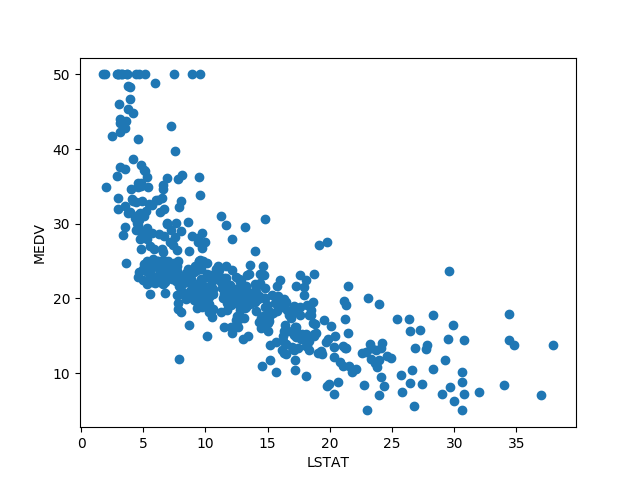
\includegraphics[width=0.4\paperwidth]{scatter}
	\caption{\label{fig:matlpotlib}Gráfico de dispersión}
\end{figure}